\documentclass[conference]{IEEEtran}
\IEEEoverridecommandlockouts
% The preceding line is only needed to identify funding in the first footnote. If that is unneeded, please comment it out.
\usepackage{cite}
\usepackage{amsmath,amssymb,amsfonts}
\usepackage{algorithmic}
\usepackage{graphicx}
\usepackage{textcomp}
\usepackage{xcolor}
\DeclareMathOperator*{\argmin}{\arg\!\min}

\def\BibTeX{{\rm B\kern-.05em{\sc i\kern-.025em b}\kern-.08em
    T\kern-.1667em\lower.7ex\hbox{E}\kern-.125emX}}
\begin{document}

\title{Learning Representative Vessel Trajectories Using Imitation Learning\\}

\author{\IEEEauthorblockN{1\textsuperscript{st} Anonymous Authors}
\IEEEauthorblockA{\textit{Anonymous Department} \\
\textit{Anonymous Organization}\\
Anonymous City, Anonymous Country \\
anon.email@domain.com}
}

\maketitle

\begin{abstract}
We suggest an exotic way of approaching the task of predicting vessel trajectories by trying to mimic the underlying behaviour policy of human captains. Decisions made by those experts are recorded by the AIS signals and can be fused with additional non-kinematic factors like weather conditions or surrounding ships to get a more accurate snapshot of the situation that led to chosen maneuvers. In this first draft we utilize Behaviour Cloning on a provisionally low-dimensional observation space to generate end-to-end vessel paths while incorporating time. The results are promising in terms of accuracy, learning efficiency and computational cost.
\end{abstract}

\begin{IEEEkeywords}
imitation, vessel, path prediction, reinforcement learning
\end{IEEEkeywords}

\section{Introduction}
Including a robust model that is capable of predicting accurate future vessel paths to any maritime surveillance system is very advantageous as it improves the overall situational awareness and allows the employment of additional features. In this context, the ability to generate end-to-end trajectories can be utilized in a variety of different tasks e.g. detecting anomalous ship behaviour or collision avoidance.
\par
However, building such a sophisticated model is a challenging task because real-world ship maneuvering not only depends on movement indicators (current position, speed, heading) but also on a wide range of non-kinematic factors (e.g. weather conditions, current, tides and surrounding ships). In addition to the high-dimensional and semantically varying feature space, a suitable system has to also incorporate a time component and retain low computational costs intending to potentially provide dozens of near real-time predictions in short time intervals.
\par
We approach this task from the perspective of imitation learning where an agent tries to extract and mimic the behaviour of human captains in order to generate similar or almost identical vessel trajectories. One major assumption is that learning from huge amounts historical expert decisions under certain environmental situations, the agent acquires the skill to generalize well enough to also assemble tracks based on states it did not encounter before.

\section{Imitation Learning}

\subsection{Relationship with Reinforcement Learning}
Imitation Learning is the general approach of extracting the underlying policy given a fixed dataset of expert trajectories. Those trajectories are sampled from an environment which can be  formalized as Markov Decision Process (MDP). This framework consists of an agent which observes the current state of the environment $s_t \in \mathcal{S}$ and interacts with it in discrete timesteps by choosing an appropriate action $a_t \in \mathcal{A}$ based on a policy $\pi: S \rightarrow A$. The environment then calculates the next state $s_{t+1}$ given the internal transition dynamics $p(s_{t+1} \mid s_t, a_t)$  and a scalar reward derived from a hand-crafted reward function $r(s_t, a_t)$ that indicates whether the proposed action was "good" or "bad".
\par
Solving such a sequential decision problem is typically achieved by applying Reinforcement Learning which uses the feedback of the environment (the reward signal) to improve the policy with an effort to maximize the discounted sum of future rewards. In fact, there are works in the literature that utilize Reinforcement Learning to the path following problem or predicting vessel trajectories. However those approaches either do not incorporate time or take place in the very distinct field of autonomous control. 
\par
Reinforcement Learning and Imitation Learning operate within the same mathematical framework of MDPs with the exception that in the case of Imitation Learning the reward function does not have to be provided or stays unknown. A crucial different as designing a suitable reward function by hand that implicitly defines the desired goal can be a tedious task, especially if the reward function is non-sparse and the researcher tries to "guide" the agent.

\subsection{Behaviour Cloning}
Behaviour Cloning reduces the task of imitating the behaviour of an expert to a supervised learning problem where a deep neuronal network learns to map states to actions as closely as possible to the expert policy $\pi^*$. That is to minimise the loss between actions suggested by the trained policy and the expert actions for all states encountered in the train set $(s, a^*) \sim P^*$, where $P^*(s|\pi^*)$ is the state distribution of the expert policy \cite{le2022survey}.

\begin{equation}
\argmin_\theta E_{(s,a^*) \sim P*} L(a^*, \pi_\theta(s))
\end{equation}


\cite{alvinn}

\subsection{Other Methods}
In the first iteration of this work, we focus on the utilization of Behaviour Cloning as primary method. Though it is planned to also apply more advanced and recent algorithms. Those potentially include the improved version of Behaviour Cloning known as \textit{DAgger}, Inverse Reinforcement Learning methods or algorithms from the uprising trend of Adversarial Imitation Learning.


\section{Experimental Setup}
\subsection{Extracting Trajectories from AIS Data}
For our initial approach, we take historical AIS data from the coast of Bremerhaven from every first month of the quarters of the year 2020. The process of filtering and extracting single vessel trajectories is done in conjunction with the library \textit{MovingPandas}\cite{graser2019movingpandas} and can be summarized as follows:

\begin{itemize}
    \item Remove records of ships moving too slow or too fast (speed over ground is $<3$ knots or $>=30$ knots)
    \item Extract provisionally trajectories
    \item Remove outliers based on Interquartile Range
    \item Split trajectories that have time gaps of more than 5 minutes in consecutive AIS signals
    \item Split trajectories by potential stops or anchoring (ships that stay within the same area of 15 diameters for at least 3 minutes).
    \item Remove all trajectories with a length of less than 300 meters
\end{itemize}

\begin{figure}[t]
\centerline{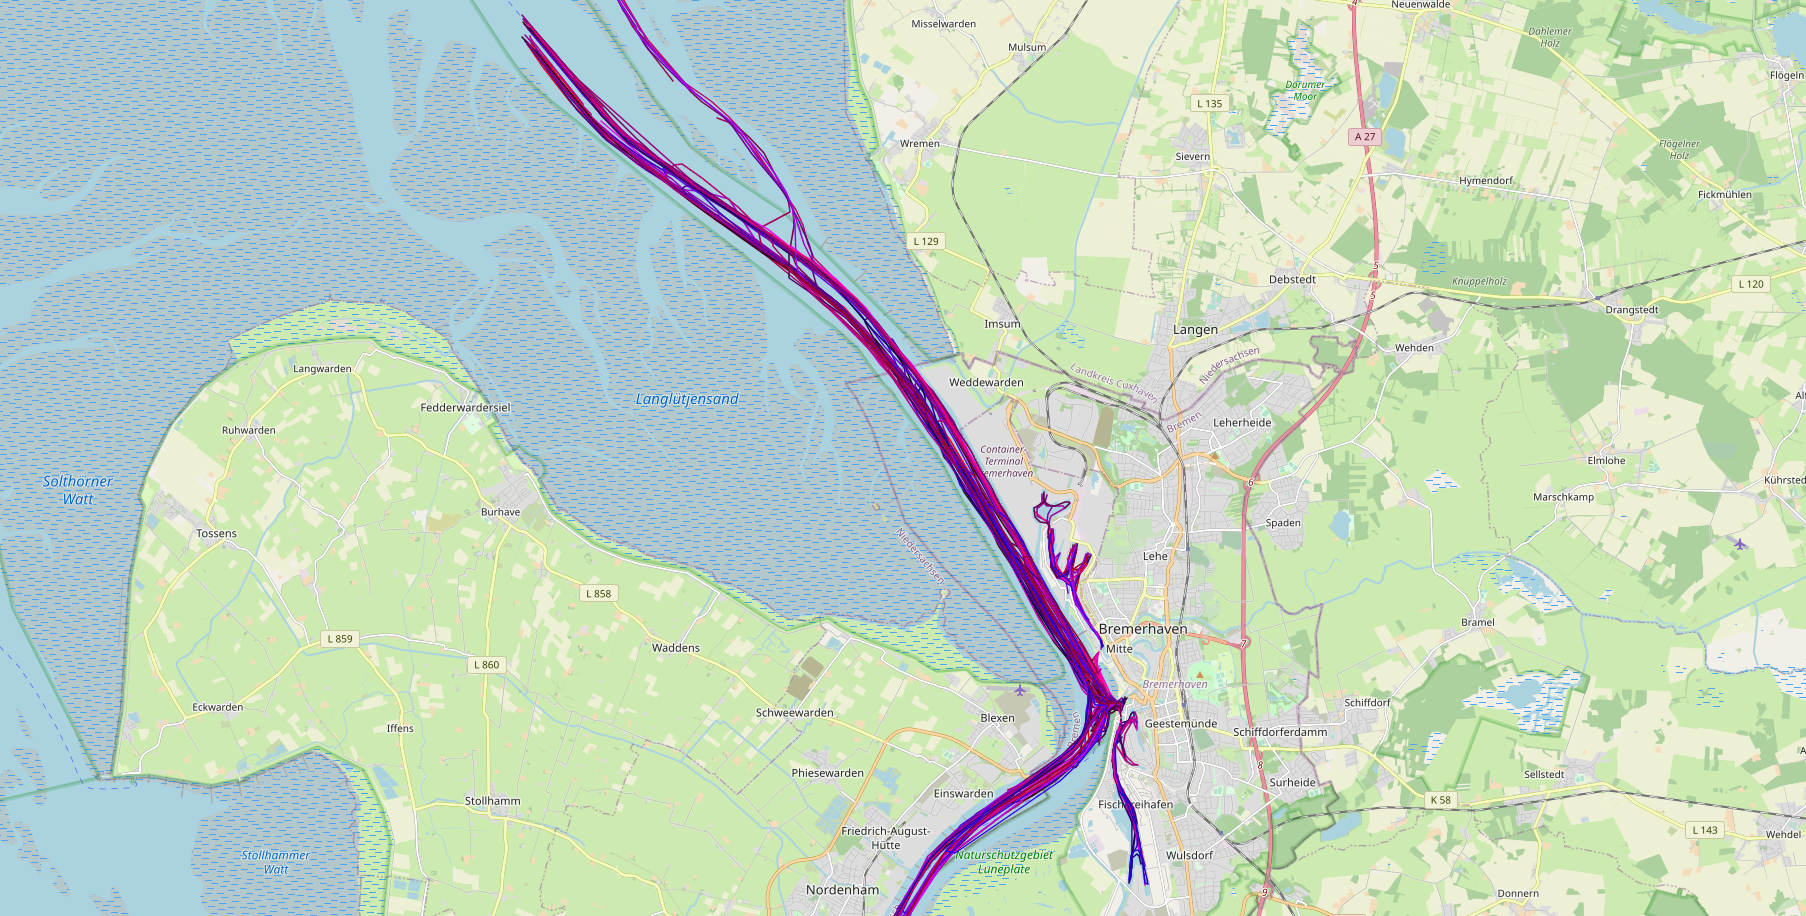
\includegraphics[width=250pt]{images/tracks.PNG}}
\caption{Example of a figure caption.}
\label{fig:tracks}
\end{figure}
The resulting dataset consists of 28,000 trajectories with a subset being shown in figure \ref{fig:tracks}. In order for the system to incorporate time, the AIS records are resampled and linear interpolated to have a fixed time interval of 5 seconds. Without explicitly knowing, the agent will always take actions that lead to the next state 5 seconds into the future.

\subsection{State Representation and Action Space}
The current draft only includes classic movement features such as position, speed and heading. Additionally, the time component is given by the fact that consecutive states are always 5 seconds apart from each other. The state- and action space can thus be defined as:
\begin{equation}
    \begin{aligned}
        \mathcal{S} &= \{lon, lat, CoG, SoG\} \\
        \mathcal{A} &= \{CoG, SoG\}
    \end{aligned}
\end{equation}

//TODO why abstract layer

\section{Results}

The close relationship between Reinforcement- and Imitation Learning also arises from the combination of those two methods. Inverse Reinforcement Learning for example first reconstructs an artificial reward function purely from the expert transition tuples $\{s_t, a_t, s_{t+1}, terminal\}$, to then apply classic interactive Reinforcement Learning. Methods like DAgger use an iterative approach of interacting with the environment while having access to the expert policy as backup.
\par

Inverse Reinforcement Learning methods like AIRL for example first reconstructs an artificial reward function purely from the expert transition tuples, to then apply classic interactive Reinforcement Learning. Furthermore improved versions of Behaviour Cloning like DAgger can be tested.

\begin{figure}[t]
\centerline{\includegraphics{fig1.png}}
\caption{Example of a figure caption.}
\label{fig}
\end{figure}
\section{Conclusion}


\bibliographystyle{IEEEtran}
\bibliography{sources}

\end{document}
